\PassOptionsToPackage{unicode=true}{hyperref} % options for packages loaded elsewhere
\PassOptionsToPackage{hyphens}{url}
\PassOptionsToPackage{dvipsnames,svgnames*,x11names*}{xcolor}
%
\documentclass[ignorenonframetext,]{beamer}
\setbeamertemplate{caption}[numbered]
\setbeamertemplate{caption label separator}{: }
\setbeamercolor{caption name}{fg=normal text.fg}
\beamertemplatenavigationsymbolsempty
\usepackage{lmodern}
\usepackage{amssymb,amsmath}
\usepackage{ifxetex,ifluatex}
\usepackage{fixltx2e} % provides \textsubscript
\ifnum 0\ifxetex 1\fi\ifluatex 1\fi=0 % if pdftex
  \usepackage[T1]{fontenc}
  \usepackage[utf8]{inputenc}
  \usepackage{textcomp} % provides euro and other symbols
\else % if luatex or xelatex
  \usepackage{unicode-math}
  \defaultfontfeatures{Ligatures=TeX,Scale=MatchLowercase}
\fi
% use upquote if available, for straight quotes in verbatim environments
\IfFileExists{upquote.sty}{\usepackage{upquote}}{}
% use microtype if available
\IfFileExists{microtype.sty}{%
\usepackage[]{microtype}
\UseMicrotypeSet[protrusion]{basicmath} % disable protrusion for tt fonts
}{}
\IfFileExists{parskip.sty}{%
\usepackage{parskip}
}{% else
\setlength{\parindent}{0pt}
\setlength{\parskip}{6pt plus 2pt minus 1pt}
}
\usepackage{xcolor}
\usepackage{hyperref}
\hypersetup{
            pdftitle={Estimation with Event-Time Data},
            pdfauthor={Dave Harrington},
            colorlinks=true,
            linkcolor=darkblue,
            citecolor=darkblue,
            urlcolor=darkblue,
            breaklinks=true}
\urlstyle{same}  % don't use monospace font for urls
\newif\ifbibliography
\usepackage{color}
\usepackage{fancyvrb}
\newcommand{\VerbBar}{|}
\newcommand{\VERB}{\Verb[commandchars=\\\{\}]}
\DefineVerbatimEnvironment{Highlighting}{Verbatim}{commandchars=\\\{\}}
% Add ',fontsize=\small' for more characters per line
\usepackage{framed}
\definecolor{shadecolor}{RGB}{248,248,248}
\newenvironment{Shaded}{\begin{snugshade}}{\end{snugshade}}
\newcommand{\AlertTok}[1]{\textcolor[rgb]{0.94,0.16,0.16}{#1}}
\newcommand{\AnnotationTok}[1]{\textcolor[rgb]{0.56,0.35,0.01}{\textbf{\textit{#1}}}}
\newcommand{\AttributeTok}[1]{\textcolor[rgb]{0.77,0.63,0.00}{#1}}
\newcommand{\BaseNTok}[1]{\textcolor[rgb]{0.00,0.00,0.81}{#1}}
\newcommand{\BuiltInTok}[1]{#1}
\newcommand{\CharTok}[1]{\textcolor[rgb]{0.31,0.60,0.02}{#1}}
\newcommand{\CommentTok}[1]{\textcolor[rgb]{0.56,0.35,0.01}{\textit{#1}}}
\newcommand{\CommentVarTok}[1]{\textcolor[rgb]{0.56,0.35,0.01}{\textbf{\textit{#1}}}}
\newcommand{\ConstantTok}[1]{\textcolor[rgb]{0.00,0.00,0.00}{#1}}
\newcommand{\ControlFlowTok}[1]{\textcolor[rgb]{0.13,0.29,0.53}{\textbf{#1}}}
\newcommand{\DataTypeTok}[1]{\textcolor[rgb]{0.13,0.29,0.53}{#1}}
\newcommand{\DecValTok}[1]{\textcolor[rgb]{0.00,0.00,0.81}{#1}}
\newcommand{\DocumentationTok}[1]{\textcolor[rgb]{0.56,0.35,0.01}{\textbf{\textit{#1}}}}
\newcommand{\ErrorTok}[1]{\textcolor[rgb]{0.64,0.00,0.00}{\textbf{#1}}}
\newcommand{\ExtensionTok}[1]{#1}
\newcommand{\FloatTok}[1]{\textcolor[rgb]{0.00,0.00,0.81}{#1}}
\newcommand{\FunctionTok}[1]{\textcolor[rgb]{0.00,0.00,0.00}{#1}}
\newcommand{\ImportTok}[1]{#1}
\newcommand{\InformationTok}[1]{\textcolor[rgb]{0.56,0.35,0.01}{\textbf{\textit{#1}}}}
\newcommand{\KeywordTok}[1]{\textcolor[rgb]{0.13,0.29,0.53}{\textbf{#1}}}
\newcommand{\NormalTok}[1]{#1}
\newcommand{\OperatorTok}[1]{\textcolor[rgb]{0.81,0.36,0.00}{\textbf{#1}}}
\newcommand{\OtherTok}[1]{\textcolor[rgb]{0.56,0.35,0.01}{#1}}
\newcommand{\PreprocessorTok}[1]{\textcolor[rgb]{0.56,0.35,0.01}{\textit{#1}}}
\newcommand{\RegionMarkerTok}[1]{#1}
\newcommand{\SpecialCharTok}[1]{\textcolor[rgb]{0.00,0.00,0.00}{#1}}
\newcommand{\SpecialStringTok}[1]{\textcolor[rgb]{0.31,0.60,0.02}{#1}}
\newcommand{\StringTok}[1]{\textcolor[rgb]{0.31,0.60,0.02}{#1}}
\newcommand{\VariableTok}[1]{\textcolor[rgb]{0.00,0.00,0.00}{#1}}
\newcommand{\VerbatimStringTok}[1]{\textcolor[rgb]{0.31,0.60,0.02}{#1}}
\newcommand{\WarningTok}[1]{\textcolor[rgb]{0.56,0.35,0.01}{\textbf{\textit{#1}}}}
\usepackage{graphicx,grffile}
\makeatletter
\def\maxwidth{\ifdim\Gin@nat@width>\linewidth\linewidth\else\Gin@nat@width\fi}
\def\maxheight{\ifdim\Gin@nat@height>\textheight\textheight\else\Gin@nat@height\fi}
\makeatother
% Scale images if necessary, so that they will not overflow the page
% margins by default, and it is still possible to overwrite the defaults
% using explicit options in \includegraphics[width, height, ...]{}
\setkeys{Gin}{width=\maxwidth,height=\maxheight,keepaspectratio}
% Prevent slide breaks in the middle of a paragraph:
\widowpenalties 1 10000
\raggedbottom
\setbeamertemplate{part page}{
\centering
\begin{beamercolorbox}[sep=16pt,center]{part title}
  \usebeamerfont{part title}\insertpart\par
\end{beamercolorbox}
}
\setbeamertemplate{section page}{
\centering
\begin{beamercolorbox}[sep=12pt,center]{part title}
  \usebeamerfont{section title}\insertsection\par
\end{beamercolorbox}
}
\setbeamertemplate{subsection page}{
\centering
\begin{beamercolorbox}[sep=8pt,center]{part title}
  \usebeamerfont{subsection title}\insertsubsection\par
\end{beamercolorbox}
}
\AtBeginPart{
  \frame{\partpage}
}
\AtBeginSection{
  \ifbibliography
  \else
    \frame{\sectionpage}
  \fi
}
\AtBeginSubsection{
  \frame{\subsectionpage}
}
\setlength{\emergencystretch}{3em}  % prevent overfull lines
\providecommand{\tightlist}{%
  \setlength{\itemsep}{0pt}\setlength{\parskip}{0pt}}
\setcounter{secnumdepth}{0}

% set default figure placement to htbp
\makeatletter
\def\fps@figure{htbp}
\makeatother


\usepackage{amsmath,verbatim}

\usepackage{fancyvrb}
\usepackage{manfnt}
\usepackage[normalem]{ulem}

%\usepackage[colorlinks=true]{hyperref}

\mode<presentation>{\usetheme{Malmoe}}

%\synctex=1

\setbeamertemplate{headline}{}


\setbeamerfont{footline}{size=\scriptsize}
\setbeamerfont{frametitle}{shape=\scshape}
\setbeamertemplate{itemize items}[circle]
\setbeamercovered{transparent}

\setbeamertemplate{navigation symbols}{}
\setbeamertemplate{footline}[frame number]{} 


\definecolor{forest}{rgb}{0, .5, 0}
\definecolor{brick}{rgb}{.5, 0, 0}
\definecolor{darkgreen}{rgb}{0, .5, 0}
\definecolor{darkred}{rgb}{.7, .15, .15}
\definecolor{darkblue}{rgb}{0, 0, .5}
\definecolor{Green}{rgb}{0.2,1,0.2}


\newcommand{\R}{\textsf{R}}
\newcommand{\RStudio}{\textsl{R Studio}}
\newcommand{\var}{\mbox{Var}}
\newcommand{\Cov}{\mbox{Cov}}
\newcommand{\Cor}{\mbox{Cor}}
\newcommand{\cip}{\mbox{$\perp\!\!\!\perp$}}
\newcommand{\bpsi}{\mbox{\boldmath$\psi$}}
\newcommand{\bbeta}{\mbox{\boldmath$\beta$}}
\newcommand{\bhat}{\mbox{\boldmath$\hat\beta$}}
\newcommand{\btheta}{\mbox{\boldmath$\theta$}}
\newcommand{\beeta}{\mbox{\boldmath$\eta$}}
\newcommand{\bfeta}{\mbox{\boldmath$\eta$}}
\newcommand{\bpsinot}{\mbox{\boldmath{$\psi_0$}}}
\newcommand{\bZ}{\bf Z}

%\usepackage[english]{babel}
\usepackage{lmodern}
\renewcommand\ttfamily{\usefont{T1}{lmtt}{m}{n}}

%\usepackage{palatino}
\usepackage[T1]{fontenc}
%\usepackage[lmodern]{babel}

% make all tt fonts bold to look more like Verbatim
\renewcommand\ttfamily{\usefont{T1}{lmtt}{m}{n}}

% Comment these out if you don't want a slide with just the
% part/section/subsection/subsubsection title:
\AtBeginPart{
  \let\insertpartnumber\relax
  \let\partname\relax
  \frame{\partpage}
}
\AtBeginSection{
  \let\insertsectionnumber\relax
  \let\sectionname\relax
  \frame{\sectionpage}
}
\AtBeginSubsection{
  \let\insertsubsectionnumber\relax
  \let\subsectionname\relax
  \frame{\subsectionpage}
}

\begin{comment}

%reduces space between code chunk and output
\usepackage{etoolbox}
\setlength{\parskip}{0pt}
\setlength{\OuterFrameSep}{0pt}
\makeatletter
\preto{\@verbatim}{\topsep=-10pt \partopsep=10pt }
\makeatother

\end{comment}

\title{Estimation with Event-Time Data}
\author{Dave Harrington}
\date{May 14 - 18, 2018}

\begin{document}
\frame{\titlepage}

\begin{frame}
\tableofcontents[hideallsubsections]
\end{frame}
\hypertarget{the-kaplan-meier-estimator}{%
\section{The Kaplan-Meier estimator}\label{the-kaplan-meier-estimator}}

\begin{frame}{%
\protect\hypertarget{approaches-to-estimating-st}{%
Approaches to estimating \(S(t)\)}}

\begin{itemize}
\item
  Parametric models and maximum likelihood
\item
  \emph{The non-parametric Kaplan-Meier (KM) estimate}

  \begin{itemize}
  \tightlist
  \item
    KM also called the product limit estimator because of original
    derivation
  \end{itemize}
\end{itemize}

\end{frame}

\begin{frame}{%
\protect\hypertarget{the-kaplan-meier-estimator-general-idea}{%
The Kaplan-Meier Estimator: General idea}}

The Kaplan-Meier estimator is probably the most popular approach.

When there is no censoring, the general formula is: \[
\widehat{S}(t) = \frac{\#~individuals~ with~T >  t}{total~sample~size}
\]

\end{frame}

\begin{frame}{%
\protect\hypertarget{an-example-cox-and-oakes-no-censoring}{%
An example: Cox and Oakes, no censoring}}

\emph{Time to relapse} (weeks) for 21 leukemia patients receiving
control treatment\footnote{Table 1.1 of Cox \& Oakes, 1984}:

\begin{itemize}
\tightlist
\item
  1, 1, 2, 2, 3, 4, 4, 5, 5, 8, 8, 8, 8, 11, 11, 12, 12, 15, 17, 22, 23
\end{itemize}

What is \(\widehat{S}(10) = \widehat{P}(T > 10)\), the probability that
an individual survives more than 10 weeks?

\begin{itemize}
\tightlist
\item
  This is 8/21 = 0.38 since 8 people survive more than 10 weeks.
\end{itemize}

What about \(\widehat{S}(8)\)?

\begin{itemize}
\tightlist
\item
  \(\widehat{S}(8) = \widehat P(T > 8) = 8/21 = 0.38\)
\item
  The four events at \(t = 8\) are counted as having already failed.
\end{itemize}

\end{frame}

\begin{frame}{%
\protect\hypertarget{empirical-survival-function}{%
Empirical survival function}}

When there is no censoring, the general formula is: \begin{align*}
\widehat{S}(t) = \frac{\#~individuals~ with~T > t}
       {total~sample~size}
\end{align*}

What is the standard error of \(\widehat{S}(t)\)?

\begin{itemize}
\tightlist
\item
  When there is no censoring, the estimated survival function is a
  proportion \(\hat{p}\) with the standard error: \[
  \text{s.e.}[\widehat{S}(t)] = \sqrt{p(1-p)/n}
  \]
\end{itemize}

\[\text{Example: s.e.}[\widehat{S}(8)]= \sqrt{(0.38)(0.62)/21} = 0.106 \]

\end{frame}

\begin{frame}{%
\protect\hypertarget{a-table-of-widehatst}{%
A table of \(\widehat{S}(t)\)}}

\begin{center}
\begin{tabular}{c|c|c}
Values of t & \# individuals with $T > t$ & ~~~~$\widehat{S}(t)$~~~~ \\
\hline
$0 \leq t < 1 $  & 21 & 21/21=1.000 \\
$1 \leq t < 2 $  & 19 & 19/21=0.905\\
$2 \leq t < 3 $  & 17 & 17/21=0.809\\
$3 \leq t < 4 $  & 16 & 16/21=0.762\\
$4 \leq t < 5 $  & 14 & 14/21=0.667\\
$5 \leq t < 8 $  & 12 & 12/21=0.571\\
$8 \leq t < 11 $ & 8 & 8/21=0.381\\ 
$11 \leq t < 12 $ & 6 & 6/21=0.286\\
$12 \leq t < 15 $ & 5 & 4/21=0.191\\
$15 \leq t < 17 $ & 3 & 3/21=0.143\\
$17 \leq t < 22 $ & 2 & 2/21=0.095\\
$22 \leq t < 23 $ & 1 & 1/21=0.048\\
\end{tabular}
\end{center}

\end{frame}

\begin{frame}{%
\protect\hypertarget{what-about-censoring}{%
What about censoring?}}

Consider time to relapse (weeks) for leukemia patients in the treatment
group.\footnote{Table 1.1 of Cox and Oakes} Times with \(^+\) are right
censored: \[6^+,6,6,6,7,9^+,10^+,10,11^+,13,16,17^+\]
\[19^+,20^+,22,23,25^+,32^+,32^+,34^+,35^+\]

Naturally, \(\widehat{S}(6-)= 21/21\)

\begin{itemize}
\tightlist
\item
  because everyone survived until at least time 6 or greater
\end{itemize}

Not right to claim \(\widehat{S}(6) = 17/21\)

\begin{itemize}
\tightlist
\item
  due to unknown status of person censored at time 6
\end{itemize}

\end{frame}

\begin{frame}{%
\protect\hypertarget{censoring-with-the-kaplan-meier}{%
Censoring with the Kaplan-Meier}}

In a 1958 paper in the \emph{Journal of the American Statistical
Association}, Kaplan and Meier proposed a way to nonparametrically
estimate \(S(t)\), in the presence of censoring.

The method is based on the ideas of \emph{conditional probability}.

\end{frame}

\begin{frame}{%
\protect\hypertarget{censoring-and-the-km-estimator}{%
Censoring and the KM estimator}}

\(S(t)\) in the discrete case:

To estimate \(S(t)\) for time \(t\) within the interval \(t_k\) and
\(t_{k+1}\), e.g. \(t_k \leq t < t_{k+1}\), consider the intervals
defined by the ordered \(k\) failure times, \[ 
[t_{0}, t_{1}), [t_{1}, t_{2}), \ldots, [t_{k-1}, t_{k}), [t_{k}, \infty)
\]

The KM estimate is constructed based on events within each interval
\([t_{j}, t_{j+1})\)

\begin{itemize}
\item
  \(d_j\) is the number of deaths in the interval \([t_{j}, t_{j+1})\)
\item
  \(r_j\) is the number of individuals at risk in the interval
  \([t_{j}, t_{j+1})\)
\end{itemize}

Initial assumptions: \(t_0=0, \;\; P(T > t_0) = 1.\)

\end{frame}

\begin{frame}{%
\protect\hypertarget{censoring-and-the-km-discrete-case}{%
Censoring and the KM: discrete case}}

Then,

\begin{align*}
S(t)=  P(T >t) &=  P(T > t_{k}) \\
   &=  P(T >  t_1, T > t_2,\ldots,T >  t_{k})\\
   &=  P(T >  t_1) \times \prod_{j=2}^k \, P(T >  t_{j}|T >  t_{j-1}) \\
&\stackrel{(*)}{=}  \prod_{j=1}^k \, [1-P(T=t_j|T >  t_{j-1})] = \prod_{j=1}^k \, [1-\lambda_j]\\
\mbox{so}~~~ \widehat{S}(t) &\cong  \prod_{j=1}^k \, \left(1-\frac{d_j}{r_j}\right) =
\prod_{j:t_j \leq t}\left(1-\frac{d_j}{r_j}\right)
\end{align*}

\footnotesize

(*) Initial assumptions: \(t_0=0, \;\; P(T > t_0)=1.\)

\end{frame}

\begin{frame}{%
\protect\hypertarget{censoring-and-the-km-continuous-case}{%
Censoring and the KM: continuous case}}

For continuous data, the Kaplan-Meier estimator of the survivorship
function \(S(t)=P(T > t)\) is \[
\widehat{S}(t) = \prod_{j: \tau_j \leq t} \frac{ r_j - d_j } {r_j}
= \prod_{j: \tau_j \leq t} \left(1 - \frac{d_j}{r_j}\right), \text{where}
\]

\begin{itemize}
\tightlist
\item
  \(\tau_1, \ldots, \tau_K\) are the K distinct death times observed
\item
  \(d_j\) is the number of deaths at \(\tau_j\)
\item
  \(r_j\) is the number of individuals ``at risk’’ right before the
  \(j\)-th death time (everyone dead or censored \emph{at or after} that
  time).

  \begin{itemize}
  \tightlist
  \item
    \(r_j = r_{j-1} - d_{j-1} - c_{j-1}\)
  \item
    Alternatively, \(r_j = \sum_{l \ge j}(c_l+d_l)\)
  \end{itemize}
\item
  \(c_j\) is the number of censored observations between the \(j\)-th
  and \((j+1)\)-th death times.

  \begin{itemize}
  \tightlist
  \item
    Censorings tied at \(\tau_j\) are included in \(c_j\)
  \end{itemize}
\end{itemize}

\end{frame}

\begin{frame}{%
\protect\hypertarget{computing}{%
Computing}}

Most widely used software packages (SAS, Stata, R) have modules for
survival analysis.

We will focus on R since it is free and has very good survival routines
written by Terry Therneau.

\end{frame}

\begin{frame}[fragile]{%
\protect\hypertarget{fitting-a-kaplan-meier-in-r}{%
Fitting a Kaplan-Meier in R}}

\scriptsize

\begin{Shaded}
\begin{Highlighting}[]
\KeywordTok{library}\NormalTok{(survival)}
\KeywordTok{library}\NormalTok{(eventtimedata)}
\KeywordTok{data}\NormalTok{(}\StringTok{"cox.oakes.leukemia"}\NormalTok{)}
\NormalTok{leukemia.remission <-}\StringTok{ }\KeywordTok{survfit}\NormalTok{(}\KeywordTok{Surv}\NormalTok{(time, relapse) }\OperatorTok{~}\StringTok{ }\NormalTok{group, }
                              \DataTypeTok{data =}\NormalTok{ cox.oakes.leukemia)}
\KeywordTok{plot}\NormalTok{(leukemia.remission, }\DataTypeTok{lty =} \DecValTok{2}\OperatorTok{:}\DecValTok{3}\NormalTok{, }\DataTypeTok{mark.time =} \OtherTok{TRUE}\NormalTok{, }\DataTypeTok{xlab =} \StringTok{"Weeks"}\NormalTok{, }
     \DataTypeTok{ylab =} \StringTok{"Survival Function"}\NormalTok{ )}
\end{Highlighting}
\end{Shaded}

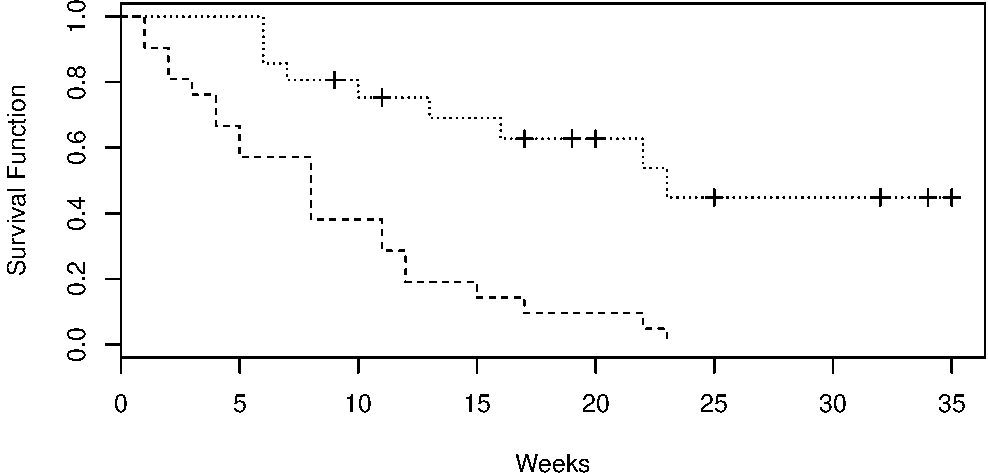
\includegraphics{unit_02_estimation_files/figure-beamer/unnamed-chunk-1-1.pdf}

\end{frame}

\begin{frame}[fragile]{%
\protect\hypertarget{numerical-output}{%
Numerical output}}

\footnotesize

\begin{Shaded}
\begin{Highlighting}[]
\KeywordTok{library}\NormalTok{(survival)}
\KeywordTok{library}\NormalTok{(eventtimedata)}
\KeywordTok{print}\NormalTok{(leukemia.remission)}
\end{Highlighting}
\end{Shaded}

\begin{verbatim}
## Call: survfit(formula = Surv(time, relapse) ~ group, data = cox.oakes.leukemia)
## 
##          n events median 0.95LCL 0.95UCL
## group=0 21     21      8       4      12
## group=1 21      9     23      16      NA
\end{verbatim}

\end{frame}

\begin{frame}[fragile]{%
\protect\hypertarget{km-numerical-estimates-group-0}{%
KM numerical estimates, group == 0}}

\scriptsize

\begin{Shaded}
\begin{Highlighting}[]
\NormalTok{leukemia.group}\FloatTok{.0}\NormalTok{ =}\StringTok{ }\KeywordTok{subset.data.frame}\NormalTok{(cox.oakes.leukemia, group }\OperatorTok{==}\StringTok{ }\DecValTok{0}\NormalTok{)}
\NormalTok{km.group}\FloatTok{.0}\NormalTok{ =}\StringTok{ }\KeywordTok{survfit}\NormalTok{(}\KeywordTok{Surv}\NormalTok{(time, relapse) }\OperatorTok{~}\StringTok{ }\DecValTok{1}\NormalTok{, }\DataTypeTok{data =}\NormalTok{ leukemia.group}\FloatTok{.0}\NormalTok{)}

\KeywordTok{summary}\NormalTok{(km.group}\FloatTok{.0}\NormalTok{)}
\end{Highlighting}
\end{Shaded}

\begin{verbatim}
## Call: survfit(formula = Surv(time, relapse) ~ 1, data = leukemia.group.0)
## 
##  time n.risk n.event survival std.err lower 95% CI upper 95% CI
##     1     21       2   0.9048  0.0641      0.78754        1.000
##     2     19       2   0.8095  0.0857      0.65785        0.996
##     3     17       1   0.7619  0.0929      0.59988        0.968
##     4     16       2   0.6667  0.1029      0.49268        0.902
##     5     14       2   0.5714  0.1080      0.39455        0.828
##     8     12       4   0.3810  0.1060      0.22085        0.657
##    11      8       2   0.2857  0.0986      0.14529        0.562
##    12      6       2   0.1905  0.0857      0.07887        0.460
##    15      4       1   0.1429  0.0764      0.05011        0.407
##    17      3       1   0.0952  0.0641      0.02549        0.356
##    22      2       1   0.0476  0.0465      0.00703        0.322
##    23      1       1   0.0000     NaN           NA           NA
\end{verbatim}

\end{frame}

\begin{frame}[fragile]{%
\protect\hypertarget{km-numerical-estimates-group-1}{%
KM numerical estimates, group == 1}}

\scriptsize

\begin{Shaded}
\begin{Highlighting}[]
\NormalTok{leukemia.group}\FloatTok{.1}\NormalTok{ =}\StringTok{ }\KeywordTok{subset.data.frame}\NormalTok{(cox.oakes.leukemia, group }\OperatorTok{==}\StringTok{ }\DecValTok{1}\NormalTok{)}
\NormalTok{km.group}\FloatTok{.1}\NormalTok{ =}\StringTok{ }\KeywordTok{survfit}\NormalTok{(}\KeywordTok{Surv}\NormalTok{(time, relapse) }\OperatorTok{~}\StringTok{ }\DecValTok{1}\NormalTok{, }\DataTypeTok{data =}\NormalTok{ leukemia.group}\FloatTok{.1}\NormalTok{)}

\KeywordTok{summary}\NormalTok{(km.group}\FloatTok{.1}\NormalTok{)}
\end{Highlighting}
\end{Shaded}

\begin{verbatim}
## Call: survfit(formula = Surv(time, relapse) ~ 1, data = leukemia.group.1)
## 
##  time n.risk n.event survival std.err lower 95% CI upper 95% CI
##     6     21       3    0.857  0.0764        0.720        1.000
##     7     17       1    0.807  0.0869        0.653        0.996
##    10     15       1    0.753  0.0963        0.586        0.968
##    13     12       1    0.690  0.1068        0.510        0.935
##    16     11       1    0.627  0.1141        0.439        0.896
##    22      7       1    0.538  0.1282        0.337        0.858
##    23      6       1    0.448  0.1346        0.249        0.807
\end{verbatim}

\normalsize

\vspace{1cm}

Subsets used here only to fit output on slides.

\texttt{summary(leukemia.remission)} prints values for both groups.

\end{frame}

\hypertarget{estimating-standard-errors}{%
\section{Estimating standard errors}\label{estimating-standard-errors}}

\begin{frame}{%
\protect\hypertarget{pointwise-confidence-intervals-for-the-km}{%
Pointwise confidence intervals for the KM}}

Why \emph{pointwise}?

\begin{itemize}
\tightlist
\item
  Since the KM is a function of time, there is an estimate of the
  standard error (or the variance) at each time.
\end{itemize}

\emph{Greenwood’s formula} is the most commonly used estimate of the KM
standard error. \[
\widehat{\text{var}} (\widehat{S}(t)) =
[\widehat{S}(t)]^2 \, \sum_{j: \tau_j \leq t} \frac{d_j}{(r_j-d_j) r_j}
\]

Derivation given later in the slides.

\end{frame}

\begin{frame}{%
\protect\hypertarget{confidence-intervals-for-the-km}{%
Confidence intervals for the KM}}

A 95\% confidence interval could be based on \[  
\widehat{S}(t)  \pm z_{1-\alpha/2} \times \text{s.e.}[\widehat{S}(t)], 
\] with \(\text{s.e.}[\widehat{S}(t)]\) estimated using Greenwood’s
formula.

\begin{itemize}
\tightlist
\item
  However, this approach can yield values \(>1\) or \(<0\).
\end{itemize}

The better approach is to use the \emph{log-log} transformation and base
intervals around \[
L(t) = \log[-\log[S(t)]]
\]

\vspace{1cm}

\footnotesize

In \textsf{R}, use the option \texttt{conf.type = "log-log"}. The
default transformation in \textsf{R} is \(L(t) = -\log[S(t)]\).

\end{frame}

\begin{frame}{%
\protect\hypertarget{confidence-intervals}{%
Confidence intervals \ldots  }}

To transform back, use \(S(t)=\exp[-\exp[L(t)]]\).

\vspace{1cm}

Since\ldots{}

\begin{itemize}
\item
  \(0 \leq S(t) \le 1\),
\item
  \(0 \leq -\log[S(t)] < \infty\), and
\item
  \(-\infty < \log[-\log[S(t)]] < \infty,\)
\end{itemize}

the confidence interval will be in the proper range when transformed
back.

\end{frame}

\begin{frame}{%
\protect\hypertarget{log-log-approach-for-confidence-intervals}{%
Log-log approach for confidence intervals:}}

\begin{enumerate}
[1.]
\item
  Define \(L(t) = \log[-\log[S(t)]]\).
\item
  Form a 95\% confidence interval for \(L(t)\),
  \((\widehat{L}(t)-A,\widehat{L}(t)+A),\) with
  \(A= 1.96 \times \text{s.e.}[\widehat{L}(t)].\)
\item
  Apply \(S(t)=\exp[-\exp[L(t)]]\) to obtain the confidence bounds for
  the 95\% CI on \(S(t)\), \[
  \left( \exp[-e^{(\widehat{L}(t)+A)}],\exp[-e^{(\widehat{L}(t)-A)}]\right)
  \]
\item
  Substituting \(\widehat{L}(t)=\log[-\log[\widehat{S}(t)]]\) back into
  the above bounds yields confidence bounds of \[
  \left([\widehat{S}(t)]^{e^A},[\widehat{S}(t)]^{e^{-A}}\right)
  \]
\end{enumerate}

\end{frame}

\begin{frame}{%
\protect\hypertarget{confidence-intervals-for-median-survival}{%
Confidence intervals for median survival}}

The median is usually defined as

\[
    q_{0.5} = \min\{t_j: \widehat{S}(t) = 0.5\}.
\]

Other quantiles are defined similarly.

Confidence limits for median survival are based on confidence intervals
for \(S(t)\).

R uses the method due to Brookmeyer and Crowley (Biometrics 1982, 38,
29–41).\\
- SAS and other packages use this as well.

The formulas are complex and not shown here.

\end{frame}

\hypertarget{the-cumulative-hazard-estimator}{%
\section{The cumulative hazard
estimator}\label{the-cumulative-hazard-estimator}}

\begin{frame}{%
\protect\hypertarget{estimating-st-via-the-nelson-aalen-cumulative-hazard}{%
Estimating \emph{S(t)} via the Nelson-Aalen cumulative hazard}}

The cumulative hazard \(\Lambda(t)\) can be approximated by a sum over
\(j\) intervals, \[\Lambda(t) \approx \sum_{j}  \lambda_j  \Delta \]

where

\begin{itemize}
\item
  \(\lambda_j\) is the value of the hazard in the \(j^{th}\) interval
\item
  \(\Delta\) is the width of each interval
\end{itemize}

Since \(\widehat{\lambda}_j \Delta\) is approximately the probability of
having an event in an interval \(j\), conditional on having survived
until the beginning of the interval, \(\Lambda(t)\) can be approximated
further as
\[\Lambda(t) \approx \sum_{j}  \lambda_j  \Delta \approx \sum_{j} \frac{d_j}{r_j}  \]

\end{frame}

\begin{frame}{%
\protect\hypertarget{estimating-st-via-the-nelson-aalen-cumulative-hazard-1}{%
Estimating \emph{S(t)} via the Nelson-Aalen cumulative hazard \ldots}}

Thus, the \emph{Nelson-Aalen estimator} can be written as
\[\widehat{\Lambda}_{\tiny NA}(t) =  \sum_{t_j \leq t} \frac{d_j}{r_j} \]

From \(\widehat{\Lambda}_{\tiny NA}(t)\), an alternative to the KM
estimator of \(S(t)\) can be calculated:

\[  \widehat{S}_{\tiny FH}(t) = \exp[-\widehat{\Lambda}_{\tiny NA}(t)] \]

The \emph{Fleming-Harrington estimator} is generally very close to
\(\widehat{S}_{\tiny KM}(t)\).

\end{frame}

\begin{frame}{%
\protect\hypertarget{example-time-to-recidivism-rossi-1980}{%
Example: Time to recidivism, Rossi (1980)}}

Recidivism is the event of rearrest and reincarceration after release
from prison.

A randomized
study\footnote{\texttt{rossi} dataset in \texttt{eventtimedata} package.}
with 52 weeks of follow-up after randomization collected information on
the following variables:

\begin{itemize}
\item
  \texttt{fin}: Financial support vs no financial support after release
\item
  \texttt{week}: Time in weeks to either re-arrest or censoring
\item
  \texttt{arrest}: \texttt{1} = arrest during the follow-up, \texttt{0}
  = no arrest
\end{itemize}

\end{frame}

\begin{frame}[fragile]{%
\protect\hypertarget{km-of-recidivism-with-confidence-intervals}{%
KM of recidivism, with confidence intervals}}

\footnotesize

\begin{Shaded}
\begin{Highlighting}[]
\KeywordTok{library}\NormalTok{(survival)}
\KeywordTok{library}\NormalTok{(eventtimedata)}
\KeywordTok{data}\NormalTok{(}\StringTok{"rossi"}\NormalTok{)}
\NormalTok{rossi.recidivism.km <-}\StringTok{ }\KeywordTok{survfit}\NormalTok{(}\KeywordTok{Surv}\NormalTok{(week, arrest) }\OperatorTok{~}\StringTok{ }\NormalTok{fin, }
                               \DataTypeTok{data =}\NormalTok{ rossi)}
\KeywordTok{plot}\NormalTok{(rossi.recidivism.km, }\DataTypeTok{lty =} \DecValTok{2}\OperatorTok{:}\DecValTok{3}\NormalTok{, }\DataTypeTok{col =} \DecValTok{3}\OperatorTok{:}\DecValTok{4}\NormalTok{, }\DataTypeTok{mark.time =} \OtherTok{TRUE}\NormalTok{, }
     \DataTypeTok{xlab =} \StringTok{"Weeks"}\NormalTok{, }
     \DataTypeTok{ylab =} \StringTok{"Probability of Recidivism"}\NormalTok{, }
     \DataTypeTok{axes =} \OtherTok{FALSE}\NormalTok{, }
     \DataTypeTok{conf.times =} \KeywordTok{c}\NormalTok{(}\DecValTok{10}\NormalTok{,}\DecValTok{30}\NormalTok{,}\DecValTok{50}\NormalTok{),}
     \DataTypeTok{main =} \StringTok{"KM of Recidivism Probability, with Conf. Int."}\NormalTok{,}
     \DataTypeTok{cex =} \FloatTok{0.6}\NormalTok{, }\DataTypeTok{cex.main =} \FloatTok{0.8}\NormalTok{)}
\KeywordTok{axis}\NormalTok{(}\DecValTok{1}\NormalTok{)}
\KeywordTok{axis}\NormalTok{(}\DecValTok{2}\NormalTok{)}
\KeywordTok{legend}\NormalTok{(}\DecValTok{10}\NormalTok{, }\FloatTok{.5}\NormalTok{, }\KeywordTok{c}\NormalTok{(}\StringTok{"Financial Support"}\NormalTok{, }\StringTok{"No Financial Support"}\NormalTok{), }
       \DataTypeTok{lty =} \DecValTok{2}\OperatorTok{:}\DecValTok{3}\NormalTok{, }\DataTypeTok{col =} \DecValTok{3}\OperatorTok{:}\DecValTok{4}\NormalTok{, }\DataTypeTok{cex =} \FloatTok{0.6}\NormalTok{)}
\end{Highlighting}
\end{Shaded}

\end{frame}

\begin{frame}

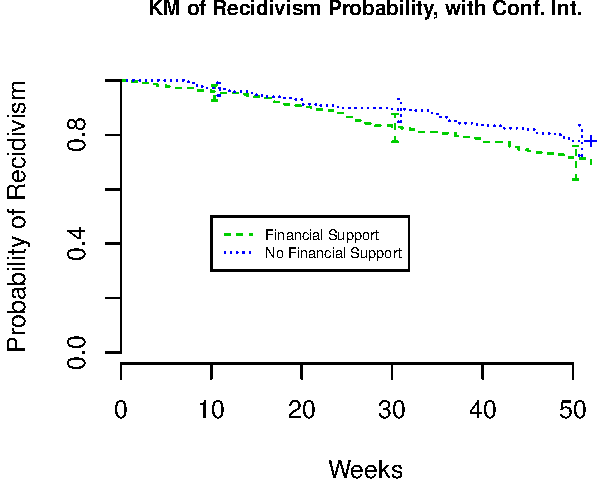
\includegraphics{unit_02_estimation_files/figure-beamer/unnamed-chunk-6-1.pdf}

\end{frame}

\begin{frame}[fragile]{%
\protect\hypertarget{cumulative-hazard-risk-of-recidivism-wcis}{%
Cumulative hazard (risk) of recidivism, w/CIs}}

\footnotesize

\begin{Shaded}
\begin{Highlighting}[]
\KeywordTok{library}\NormalTok{(survival)}
\KeywordTok{library}\NormalTok{(eventtimedata)}
\KeywordTok{data}\NormalTok{(}\StringTok{"rossi"}\NormalTok{)}
\NormalTok{rossi.recidivism.ch <-}\StringTok{ }\KeywordTok{survfit}\NormalTok{(}\KeywordTok{Surv}\NormalTok{(week, arrest) }\OperatorTok{~}\StringTok{ }\NormalTok{fin, }
                               \DataTypeTok{data =}\NormalTok{ rossi)}
\KeywordTok{plot}\NormalTok{(rossi.recidivism.km, }\DataTypeTok{lty =} \DecValTok{2}\OperatorTok{:}\DecValTok{3}\NormalTok{, }\DataTypeTok{col =} \DecValTok{3}\OperatorTok{:}\DecValTok{4}\NormalTok{, }\DataTypeTok{mark.time =} \OtherTok{TRUE}\NormalTok{, }
     \DataTypeTok{fun =} \StringTok{"cumhaz"}\NormalTok{,}
     \DataTypeTok{xlab =} \StringTok{"Weeks"}\NormalTok{, }
     \DataTypeTok{ylab =} \StringTok{"Cumulative Hazard of Recidivism"}\NormalTok{, }
     \DataTypeTok{axes =} \OtherTok{FALSE}\NormalTok{, }
     \DataTypeTok{conf.times =} \KeywordTok{c}\NormalTok{(}\DecValTok{10}\NormalTok{,}\DecValTok{30}\NormalTok{,}\DecValTok{50}\NormalTok{),}
     \DataTypeTok{main =} \StringTok{"Cumulative Risk of Recidivism Probability, }
\StringTok{     with Conf. Int."}\NormalTok{,}
     \DataTypeTok{cex =} \FloatTok{0.6}\NormalTok{, }\DataTypeTok{cex.main =} \FloatTok{0.8}\NormalTok{)}
\KeywordTok{axis}\NormalTok{(}\DecValTok{1}\NormalTok{)}
\KeywordTok{axis}\NormalTok{(}\DecValTok{2}\NormalTok{)}
\KeywordTok{legend}\NormalTok{(}\StringTok{"topleft"}\NormalTok{, }\DataTypeTok{inset =} \KeywordTok{c}\NormalTok{(}\FloatTok{0.1}\NormalTok{, }\FloatTok{0.3}\NormalTok{), }
       \KeywordTok{c}\NormalTok{(}\StringTok{"Financial Support"}\NormalTok{, }\StringTok{"No Financial Support"}\NormalTok{),}
       \DataTypeTok{lty =} \DecValTok{2}\OperatorTok{:}\DecValTok{3}\NormalTok{, }\DataTypeTok{col =} \DecValTok{3}\OperatorTok{:}\DecValTok{4}\NormalTok{, }\DataTypeTok{cex =} \FloatTok{0.6}\NormalTok{)}
\end{Highlighting}
\end{Shaded}

\end{frame}

\begin{frame}

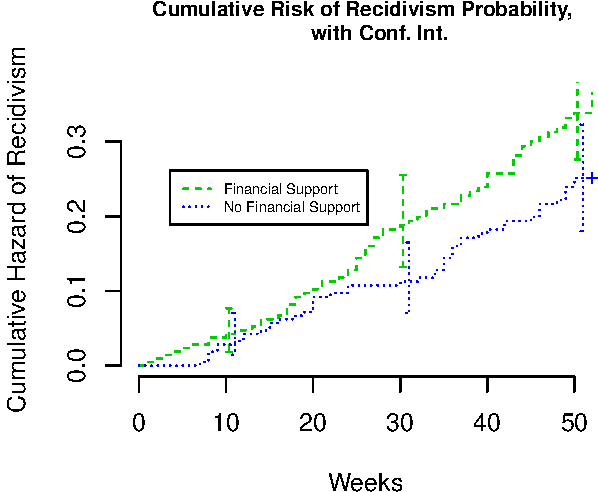
\includegraphics{unit_02_estimation_files/figure-beamer/unnamed-chunk-8-1.pdf}

\end{frame}

\begin{frame}{%
\protect\hypertarget{confidence-intervals-vs-confidence-bands}{%
Confidence intervals vs confidence bands}}

Examining many confidence intervals may cause the same problem as
simultaneous hypothesis tests.

\begin{itemize}
\tightlist
\item
  Overall coverage probability for the curve is not right.
\end{itemize}

Hall and Wellner (\emph{Biometrika}, 1980) solved that problem by
deriving confidence bands:

\begin{itemize}
\item
  95\% bands have probability 0.95 of covering the entire survival
  curve.
\item
  These bands will be wider than pointwise intervals.
\item
  Formulas complex, not shown here.
\end{itemize}

\end{frame}

\begin{frame}[fragile]{%
\protect\hypertarget{km-of-recidivism-with-confidence-bands}{%
KM of recidivism, with confidence bands}}

\footnotesize

\begin{Shaded}
\begin{Highlighting}[]
\KeywordTok{library}\NormalTok{(survival)}
\KeywordTok{library}\NormalTok{(eventtimedata)}
\KeywordTok{data}\NormalTok{(}\StringTok{"rossi"}\NormalTok{)}
\NormalTok{rossi.recidivism.km <-}\StringTok{ }\KeywordTok{survfit}\NormalTok{(}\KeywordTok{Surv}\NormalTok{(week, arrest) }\OperatorTok{~}\StringTok{ }\NormalTok{fin, }
                               \DataTypeTok{data =}\NormalTok{ rossi)}
\KeywordTok{plot}\NormalTok{(rossi.recidivism.km, }\DataTypeTok{lty =} \DecValTok{2}\OperatorTok{:}\DecValTok{3}\NormalTok{, }\DataTypeTok{col =} \DecValTok{3}\OperatorTok{:}\DecValTok{4}\NormalTok{, }\DataTypeTok{mark.time =} \OtherTok{TRUE}\NormalTok{, }
     \DataTypeTok{xlab =} \StringTok{"Weeks"}\NormalTok{, }
     \DataTypeTok{ylab =} \StringTok{"Probability of Re-arrest"}\NormalTok{, }
     \DataTypeTok{axes =} \OtherTok{FALSE}\NormalTok{, }
     \DataTypeTok{conf.int =} \OtherTok{TRUE}\NormalTok{,}
     \DataTypeTok{main =} \StringTok{"KM of Recidivism Probability, with Conf. Bands"}\NormalTok{,}
     \DataTypeTok{cex =} \FloatTok{0.6}\NormalTok{, }\DataTypeTok{cex.main =} \FloatTok{0.8}\NormalTok{)}
\KeywordTok{axis}\NormalTok{(}\DecValTok{1}\NormalTok{)}
\KeywordTok{axis}\NormalTok{(}\DecValTok{2}\NormalTok{)}
\KeywordTok{legend}\NormalTok{(}\DecValTok{10}\NormalTok{, }\FloatTok{.5}\NormalTok{, }\KeywordTok{c}\NormalTok{(}\StringTok{"Financial Support"}\NormalTok{, }\StringTok{"No Financial Support"}\NormalTok{),}
       \DataTypeTok{lty =} \DecValTok{2}\OperatorTok{:}\DecValTok{3}\NormalTok{, }\DataTypeTok{col =} \DecValTok{3}\OperatorTok{:}\DecValTok{4}\NormalTok{, }\DataTypeTok{cex =} \FloatTok{0.6}\NormalTok{)}
\end{Highlighting}
\end{Shaded}

\end{frame}

\begin{frame}

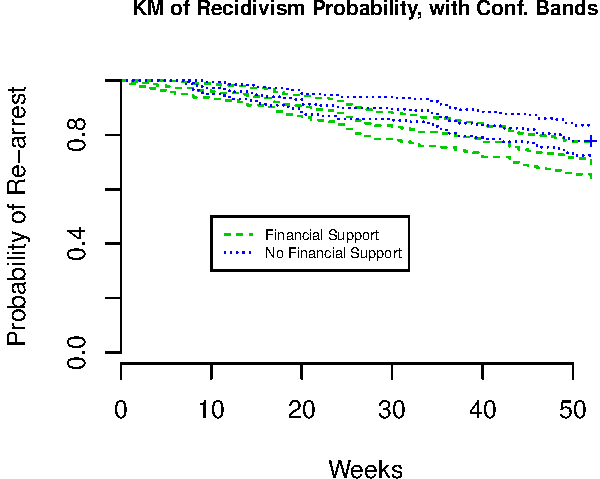
\includegraphics{unit_02_estimation_files/figure-beamer/unnamed-chunk-10-1.pdf}

\end{frame}

\begin{frame}{%
\protect\hypertarget{example-application-to-fda-7-march-2018}{%
Example: Application to FDA (7 March 2018)}}

On 7 March 2018, Amgen asked for FDA approval of the drug blinatumumab
in patients with a sub-type of acute lymphoblastic leukemia (ALL).

\begin{itemize}
\tightlist
\item
  The drug would be given to patients who experienced a clinical
  complete remission, but had evidence of minimal residual disease
  (MRD).
\end{itemize}

Figure on the next slide from the
\href{https://www.fda.gov/downloads/AdvisoryCommittees/CommitteesMeetingMaterials/Drugs/OncologicDrugsAdvisoryCommittee/UCM599298.pdf}{FDA
analysis} of the data shows

\begin{itemize}
\item
  Relapse free survival by MRD status
\item
  Shows confidence bands (Hall and Wellner)
\end{itemize}

\end{frame}

\begin{frame}

\begin{figure}
\centering
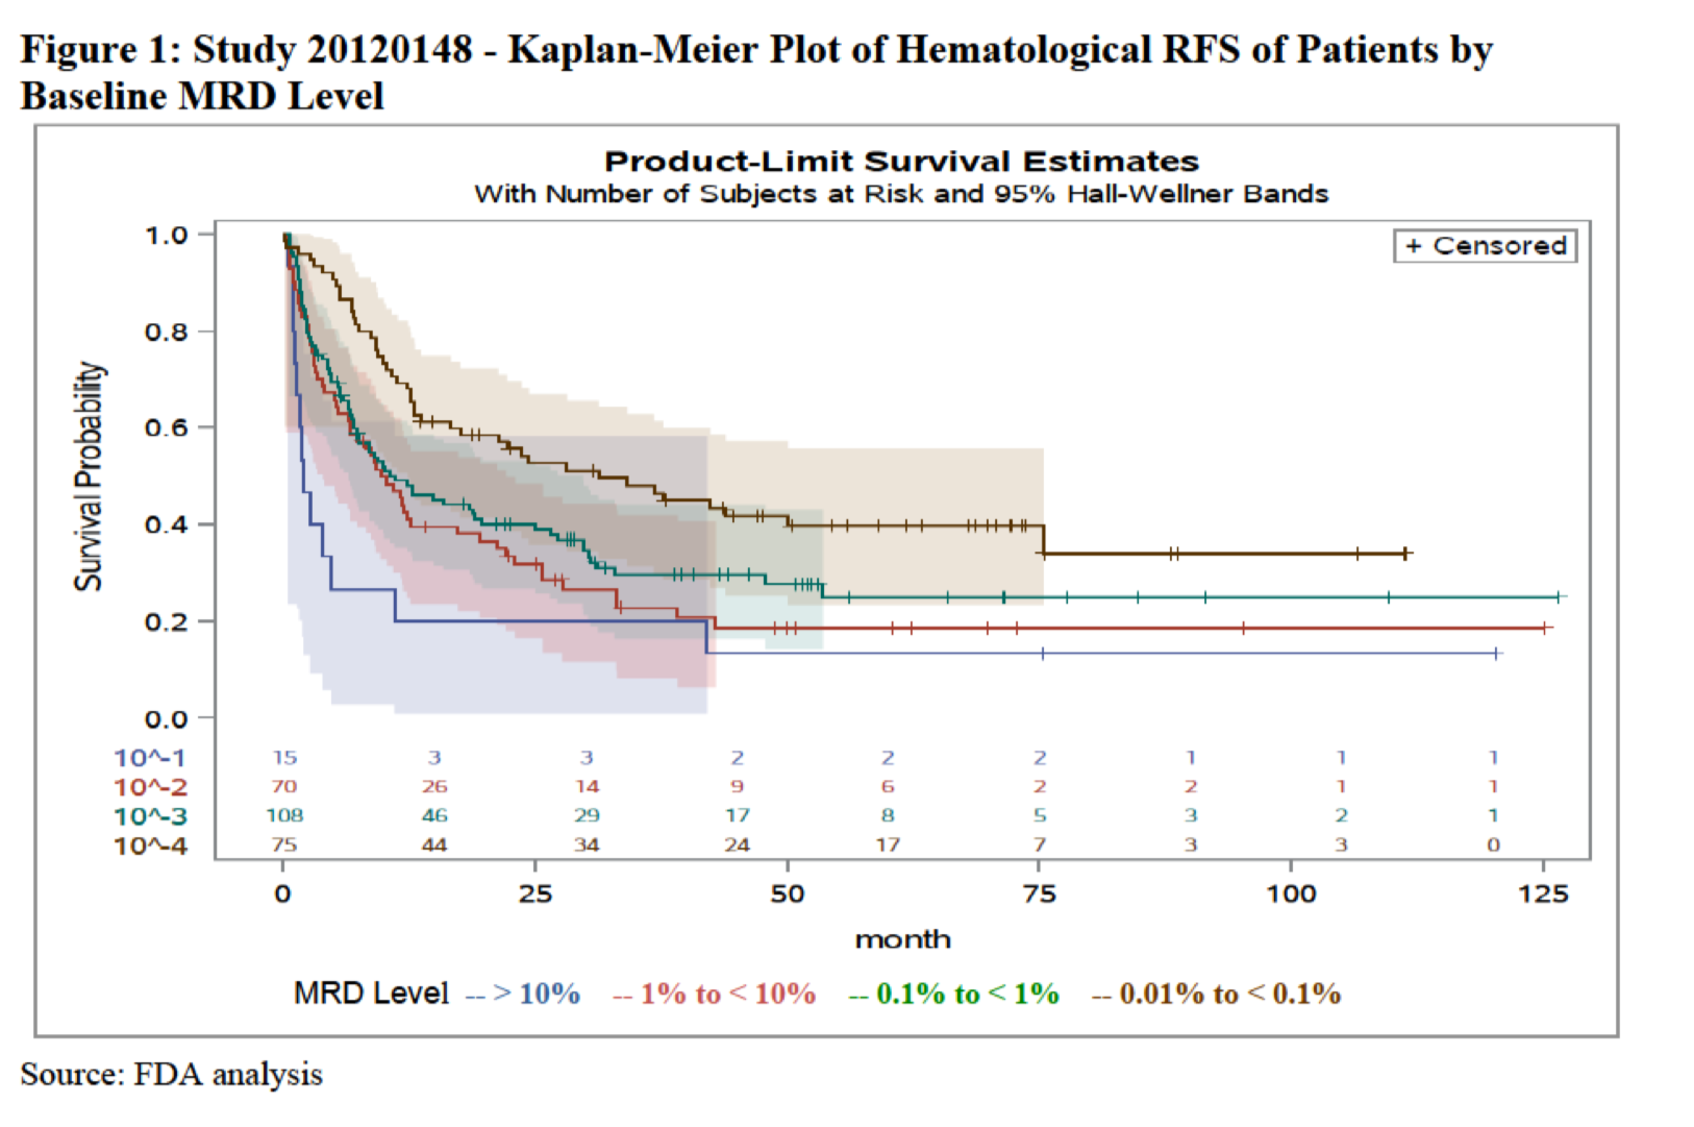
\includegraphics[width=0.9\textwidth,height=\textheight]{../figures/usfda_mrd_leukemia_km.pdf}
\caption{FDA presentation, 7 March 2018}
\end{figure}

\end{frame}

\hypertarget{derivations}{%
\section{Derivations}\label{derivations}}

\begin{frame}{%
\protect\hypertarget{km-estimator-derivation-continuous-case}{%
KM estimator derivation, continuous case \ldots}}

\emph{Conditional Probability:} Suppose \(A\) and \(B\) are two events.
Then, \[  P(A|B)  =    \frac { P(A \cap B)}  { P(B)}\]

\emph{Multiplication Law}: Multiply both sides of the above by \(P(B)\).
\[P(A \cap B) =  P(A|B) P(B) \]

\emph{Extension to more than 2 events:} Suppose
\(A_1, A_2, \ldots, A_k\) are \(k\) different events. Then, the
probability of all \(k\) events occurring can be written as a product of
conditional probabilities. \begin{align*}
P(A_1 \cap A_2 \ldots \cap A_k) =& \ P(A_k|A_{k-1} \cap \ldots \cap A_1) \\
& \qquad \times P(A_{k-1}|A_{k-2} \cap \ldots \cap A_1) \\
& \qquad \times \ldots \\
& \qquad \times P(A_2 | A_1) \\
& \qquad \times P(A_1)
\end{align*}

\[
   P(A_1 \cap A_2 ... \cap A_k)   = \]

\[ P(A_k|A_{k-1} \cap ... \cap A_1)
         \times  P(A_{k-1}|A_{k-2} \cap  ... \cap A_1) \times
              ...     \times P(A_2| A_1) \times P(A_1) .\]

\end{frame}

\begin{frame}{%
\protect\hypertarget{km-estimator-derivation-continuous-case-1}{%
KM estimator derivation, continuous case \ldots}}

Think of dividing the observed time-span of the study into a series of
small intervals so that there is a separate interval for each time of
death or censoring (with possible ties):

\begin{center}
\begin{tabular}{l|p{.4in}|p{.4in}|p{.4in}
 |p{.4in}|p{.4in}|p{.4in}|p{.4in}|p{.4in}|p{.4in}|p{.4in}
 |p{.4in}|p{.4in}|p{.4in}}
  &   &  &   & &   & &   & C &   &   \\
  &   &  & D & & C & & C & D & D & D \\  \hline
\end{tabular}
\end{center}

Using the law of conditional probability,
\[P(T > t) = \prod_j P(\text{survive $j$-th interval $I_j$ | survived to start of $I_j$}), \]
over all intervals preceding time \(t\).

\end{frame}

\begin{frame}{%
\protect\hypertarget{km-estimator-derivation-continuous-case-2}{%
KM estimator derivation, continuous case \ldots}}

\emph{Four possibilities for each interval:}

\begin{enumerate}
[1.]
\item
  No event: conditional probability of surviving the interval is 1.
\item
  Censoring: assume individual survives to end of the interval, so that
  the conditional probability of surviving the interval is 1.
\item
  Death, but no censoring: conditional probability of \emph{not}
  surviving the interval is \# deaths (\(d\)) divided by \# “at risk”
  (\(r\)) at the beginning of the interval. Thus, the conditional
  probability of surviving the interval is \(1 - \frac{d}{r}\).
\item
  Tied deaths and censoring: assume censorings survive to end of the
  interval, so that conditional probability of surviving the interval is
  still \(1 - \frac{d}{r}\).
\end{enumerate}

Thus, the general formula for the conditional probability of surviving
the \(j\)-th interval that holds for all 4 cases is
\(1-\frac{d_j}{r_j}\).

\end{frame}

\begin{frame}{%
\protect\hypertarget{km-estimator-derivation-continuous-case-3}{%
KM estimator derivation, continuous case \ldots}}

As the intervals become smaller,

\begin{itemize}
\tightlist
\item
  The approximations made in estimating the probabilities of surviving
  each interval become smaller.\\
\item
  The estimator converges to the true \(S(t)\) as the sample size
  increases.
\end{itemize}

This argument clarifies why an alternative name for the KM is the
\emph{product limit estimator}.

\end{frame}

\begin{frame}{%
\protect\hypertarget{result-stated-earlier}{%
Result stated earlier}}

For continuous data, the Kaplan-Meier estimator of the survivorship
function \(S(t)=P(T > t)\) is \[
\widehat{S}(t) = \prod_{j: \tau_j \leq t} \frac{ r_j - d_j } {r_j}
= \prod_{j: \tau_j \leq t} \left(1 - \frac{d_j}{r_j}\right), \text{where}
\]

\begin{itemize}
\tightlist
\item
  \(\tau_1, \ldots, \tau_K\) are the K distinct death times observed
\item
  \(d_j\) is the number of deaths at \(\tau_j\)
\item
  \(r_j\) is the number of individuals ``at risk’’ right before the
  \(j\)-th death time (everyone dead or censored \emph{at or after} that
  time).

  \begin{itemize}
  \tightlist
  \item
    \(r_j = r_{j-1} - d_{j-1} - c_{j-1}\)
  \item
    Alternatively, \(r_j = \sum_{l \ge j}(c_l+d_l)\)
  \end{itemize}
\item
  \(c_j\) is the number of censored observations between the \(j\)-th
  and \((j+1)\)-th death times.

  \begin{itemize}
  \tightlist
  \item
    Censorings tied at \(\tau_j\) are included in \(c_j\)
  \end{itemize}
\end{itemize}

\end{frame}

\begin{frame}{%
\protect\hypertarget{derivation-of-greenwoods-formula}{%
Derivation of Greenwood’s formula}}

KM estimator can be thought of as \[  
\widehat{S}(t) = \prod_{j: \tau_j \leq t} (1-\widehat{\lambda}_j), \text{ where } \widehat{\lambda}_j = \frac{d_j}{r_j}.
\]

Since the \(\widehat\lambda_j\)’s are (conditionally) binomial
proportions, standard likelihood theory can be used to to show each
\(\widehat{\lambda}_j\) is approximately normally distributed, with mean
\(\lambda_j\), and
variance\footnote{The estimated variance is $\widehat{\text{var}}(\widehat{\lambda}_j) = \frac{\widehat{\lambda}_j
(1-\widehat{\lambda}_j)}{r_j}$.} \[
\text{var}(\widehat{\lambda}_j) 
= \frac{{\lambda}_j (1-{\lambda}_j)}{r_j}
\]

The \(\widehat\lambda_j\)’s are independent in large enough samples.

\end{frame}

\begin{frame}{%
\protect\hypertarget{derivation-of-greenwoods-formula-1}{%
Derivation of Greenwood’s formula \ldots}}

Since \(\widehat{S}(t)\) is a function of the \(\lambda_j\)’s, its
variance can be estimated using the \emph{delta method},

\begin{itemize}
\tightlist
\item
  an approach for calculating the variance of non-linear functions.
\end{itemize}

\emph{Delta method:} If \(Y\) is normal with mean \(\mu\) and variance
\(\sigma^2\), then \(g(Y)\) is approximately normally distributed with
mean \(g(\mu)\) and variance \([g'(\mu)]^2 \sigma^2\).

\end{frame}

\begin{frame}{%
\protect\hypertarget{digression-the-delta-method}{%
Digression: the delta method}}

Two specific examples that will be used in the derivation:

\begin{itemize}
\item
  Ex. 1: \(Z = g(Y)= \log(Y)\), then \(g'(y)=(1/y)\): \[
  Z \sim N\left(\log(\mu),\left(\frac{1}{\mu}\right)^2 \sigma^2\right)
  \]
\item
  Ex. 2: \(Z = g(Y)= \exp(Y)\), then \(g'(y)=e^y\): \[
  Z \sim N\left(e^{\mu}, [e^{\mu}]^2 \sigma^2\right)
  \]
\end{itemize}

\end{frame}

\begin{frame}{%
\protect\hypertarget{derivation-of-greenwoods-formula-2}{%
Derivation of Greenwood’s formula \ldots}}

Instead of dealing with \(\widehat{S}(t)\) directly, use
\(\log[\widehat{S}(t)]\) since calculating variance of a sum is easier
than calculating variance of a product,
\[ \log[\widehat{S}(t)] = \sum_{j: \tau_j \le t} \log(1-\widehat{\lambda}_j)  \]

By approximate independence of the \(\widehat{\lambda}_j\)’s,
\[\text{var}(\log[\widehat{S}(t)]) = 
\sum_{j: \tau_j \le t} \text{var}[\log(1-\widehat{\lambda}_j)]. \]

\small

Apply the delta method (Ex. 1), where \(\mu = 1 - \lambda_j\) and
\(\sigma^2 = \frac{{\lambda}_j (1-{\lambda}_j)}{r_j}\).

\vspace{-0.4cm}

\begin{align*}
\widehat{\text{var}}(\log[\widehat{S}(t)]) =& \sum_{j: \tau_j \leq t} \left(\frac{1}{1 - \widehat{\lambda}_j} \right)^2 \left(\frac{\widehat{{\lambda}}_j (1-\widehat{{\lambda}}_j)}{r_j} \right) \\
=& \sum_{j: \tau_j \leq t} \frac{\widehat{\lambda}_j}{(1-\widehat{\lambda}_j) r_j} = \sum_{j: \tau_j \leq t} \frac{d_j}{(r_j-d_j) r_j}
\end{align*}

\end{frame}

\begin{frame}{%
\protect\hypertarget{greenwoods-formula}{%
Greenwood’s formula}}

To obtain \(\widehat{\text{var}}(\widehat{S}(t))\), apply the delta
method again (Ex. 2), using the relationship
\(\widehat{S}(t) = \exp[\log[\widehat{S}(t)]]\),
\[\widehat{\text{var}}(\widehat{S}(t)) = [\widehat{S}(t)]^2 \ \widehat{\text{var}}\left[\log[\widehat{S}(t)] \right] \]

Substitute the previous result for
\(\widehat{\text{var}}\left[\log[\widehat{S}(t)] \right]\) to obtain
Greenwood’s Formula,
\[\widehat{\text{var}}(\widehat{S}(t)) = [\widehat{S}(t)]^2  \sum_{j: \tau_j \leq t} \frac{d_j}{(r_j-d_j) r_j} \]

\end{frame}

\end{document}
